\documentclass{beamer}
%\usetheme{Boadilla}
%\usetheme{Szeged}
%\usetheme{Singapore}
%\usetheme{Frankfurt}
\usecolortheme{dove}
%\setbeamertemplate{navigation symbols}{{\footnotesize\insertframenumber}}
\setbeamertemplate{navigation symbols}{}
%\setbeamertemplate{headline}{%
  %  \leavevmode%
    %\hbox{%
    %\insertsectionnavigationhorizontal{\textwidth}{\hspace{20pt}}{\hspace{20pt}}
  %}
%}
\newenvironment{alltt}{\ttfamily}{\par}
\usepackage{amsmath,amssymb,amsfonts,amsthm, multicol, subfigure, color}
\usepackage{bm}
\usepackage{graphicx}
\usepackage{tabularx}
\usepackage{booktabs}
\usepackage{hyperref}
\usepackage{pdfpages}
\usepackage{xcolor}
\definecolor{dodgerblue}{rgb}{.118, .575, 1}
\definecolor{seagreen4}{RGB}{46, 139, 87}
\def\independenT#1#2{\mathrel{\rlap{$#1#2$}\mkern2mu{#1#2}}}
\newcommand\independent{\protect\mathpalette{\protect\independenT}{\perp}}
\newcommand\indep{\protect\mathpalette{\protect\independenT}{\perp}}
\def\logit{\text{logit}}
\usepackage{stackrel}
\usepackage{tikz}
\usetikzlibrary{arrows,shapes.arrows,positioning,shapes,patterns,calc,snakes}
\newcommand\slideref[1]{\vskip .1cm \scriptsize \textcolor{gray}{{#1}}}
\newcommand\red[1]{{\color{red}#1}}
\newcommand\bred[1]{{\color{red}\textbf{#1}}}
\newcommand\blue[1]{{\color{blue}#1}}
\newcommand\bblue[1]{{\color{blue}\textbf{#1}}}
\newcommand\gray[1]{{\color{gray}#1}}
\newcommand\bgray[1]{{\color{gray}\textbf{#1}}}
\newcommand\green[1]{{\color{seagreen4}#1}}
\newcommand\bgreen[1]{{\color{seagreen4}\textbf{#1}}}
\newcommand\purple[1]{{\color{purple}#1}}
\newcommand\orange[1]{{\color{orange}#1}}
\newcommand\black[1]{{\color{black}#1}}
\newcommand\white[1]{{\color{white}#1}}
\newcommand\teal[1]{{\color{teal}#1}}
\newcommand\magenta[1]{{\color{magenta}#1}}
\newcommand\Fuchsia[1]{{\color{Fuchsia}#1}}
\newcommand\BlueGreen[1]{{\color{BlueGreen}#1}}
\colorlet{lightgray}{gray!40}
\newcommand\bref[2]{\href{#1}{\color{blue}{#2}}}
\pgfdeclarelayer{bg}    % declare background layer for tikz
\pgfsetlayers{bg,main} % order layers for tikz
\newcommand\mycite[1]{\begin{scriptsize}\textcolor{darkgray}{(#1)}\end{scriptsize}}
\newcommand\iid{\stackrel{\text{iid}}{\sim}}
\newcommand\E{\text{E}}
\newcommand\V{\text{V}}
\renewcommand\P{\text{P}}
\newcommand{\Cov}{\text{Cov}}
\newcommand{\Cor}{\text{Cor}}
\newcommand\doop{\text{do}}
\newcommand{\tcframe}{\frame{
\small{
\only<1|handout:0>{\tableofcontents}
\only<2|handout:1>{\tableofcontents[currentsection]}}
}}
% Credit for the following to https://tex.stackexchange.com/questions/44983/beamer-removing-headline-and-its-space-on-a-single-frame-for-plan-but-keepin
\makeatletter
    \newenvironment{withoutheadline}{
        \setbeamertemplate{headline}[default]
        \def\beamer@entrycode{\vspace*{-\headheight}}
    }{}
\makeatother
\setbeamercovered{invisible}
\usepackage[round]{natbib}
\bibliographystyle{humannat-mod}
\setbeamertemplate{enumerate items}[default]
\usepackage{mathtools}
% BELOW THREE LINES MAKES NAME IN FOOTER
\setbeamertemplate{footline}[text line]{%
%\parbox{\linewidth}{\vspace*{-8pt}Ian Lundberg (Cornell)}}
\parbox{\linewidth}{\vspace*{-8pt}Ian Lundberg\hfill
\insertsectionnavigationhorizontal{.7\paperwidth}{}{\hfill\hfill}}
}
%\hfill \insertframenumber/23}}%\hfill\insertshortauthor\hfill\insertpagenumber}}
%\setbeamertemplate{navigation symbols}{}
\usepackage{framed}
\usepackage{soul}
\usepackage{appendixnumberbeamer}

\title{The gap-closing estimand: A causal approach to study interventions that close disparities across social categories}
\author{Ian Lundberg}
\date{\today}

\begin{document}

{
\setbeamertemplate{footline}[text line]{\parbox{\linewidth}{\vspace*{-8pt}Ian Lundberg (Cornell)\hfill}}
\begin{frame}
\begin{tikzpicture}[x = \textwidth, y = \textheight]
\node at (0,0) {};
\node at (1,1) {};
\node[anchor = north west, align = left, font = \Large] at (0,.9) {The \bblue{gap-closing estimand}};
\node[anchor = north west, align = left, font = \large] at (0,.8) {A causal approach
\\to study \bgreen{interventions}\\that \bgreen{close disparities}\\across social categories};
\node[anchor = north, align = center] at (.5,.55) {\bgray{Ian Lundberg}};
\node[anchor = south, align = center, font = \footnotesize] at (.5,.35) {Cornell University\\Department of Information Science\\ilundberg@cornell.edu};
\node[anchor = south, align = center, font = \footnotesize] at (.5,.25) {9 March 2023\\NJ Acts Biostatistics and Epidemiology Workshop Series};
\node[anchor = south west, align = left, font = \tiny, text width = \textwidth] at (0,.1) {Paper in \bref{https://doi.org/10.1177/00491241211055769}{\emph{Sociological Methods and Research}}. Replication code on \bref{https://doi.org/10.7910/DVN/UWYAJD}{Dataverse}. R package \bref{https://ilundberg.github.io/gapclosing/}{\texttt{gapclosing}} on \bref{https://cran.r-project.org/web/packages/gapclosing/}{CRAN}. Research reported in this publication was supported by The Eunice Kennedy Shriver National Institute of Child Health \& Human Development of the National Institutes of Health under Award Number P2CHD047879 and by the National Science Foundation under Award Number 2104607.};
\node[anchor = north east, align = right, font = \footnotesize] (slides) at (1,.9) {Slides at\\\bref{https://www.ianlundberg.org/}{ianlundberg.org}};
\node[anchor = north east, align = right, font = \footnotesize] (software) at (slides.south east) {Software at\\\bref{https://ilundberg.github.io/gapclosing/github_doc/_book/index.html}{ilundberg.github.io/gapclosing}};
%\draw[thick, gray] (slides.north west) -- (software.south west) -- (software.south east);
\end{tikzpicture}
\end{frame}

% Introduce gap-closing
\begin{frame}
\begin{tikzpicture}[x = \textwidth, y = \textheight]
\node at (0,0) {};
\node at (1,1) {};
\node[circle, fill = lightgray, draw = lightgray, font = \footnotesize, inner sep = 2pt] at (.42,.8) {\phantom{$t$}};
\node[circle, fill = lightgray, draw = lightgray, font = \footnotesize, inner sep = 2pt] at (.37,.75) {\phantom{$t$}};
\node[circle, fill = lightgray, draw = lightgray, font = \footnotesize, inner sep = 2pt] at (.42,.7) {\phantom{$t$}};
\node[diamond, fill = lightgray, draw = lightgray, font = \footnotesize, inner sep = 2pt] at (.58,.8) {\phantom{$t$}};
\node[diamond, fill = lightgray, draw = lightgray, font = \footnotesize, inner sep = 2pt] at (.63,.75) {\phantom{$t$}};
\node[diamond, fill = lightgray, draw = lightgray, font = \footnotesize, inner sep = 2pt] at (.58,.7) {\phantom{$t$}};
\only<2>{
\node[font = \bf, gray, align = center, anchor = north] (category1) at (.4,.95) {Working\\Class};
\node[font = \bf, gray, align = center, anchor = north] (category2) at (.6,.95) {Professional\\Class};
}
\only<3>{
\node[font = \bf, gray, align = center, anchor = south] (category1) at (.4,.85) {Men};
\node[font = \bf, gray, align = center, anchor = south] (category2) at (.6,.85) {Women};
}
\only<4->{
\node[font = \bf, gray, align = center, anchor = south] (category1) at (.4,.85) {Black};
\node[font = \bf, gray, align = center, anchor = south] (category2) at (.6,.85) {White};
}
% TREATED
\only<5->{
\node[anchor = east, font = \small, gray, align = center] (treatment_note) at (.3,.6) {Give everyone\\a treatment $t$};
\draw[->, thick, gray] (treatment_note) to[bend right] (.33,.51);
\node[circle, fill = lightgray, draw = lightgray, font = \footnotesize, inner sep = 2pt] at (.42,.57) {$t$};
\node[circle, fill = lightgray, draw = lightgray, font = \footnotesize, inner sep = 2pt] at (.37,.52) {$t$};
\node[circle, fill = lightgray, draw = lightgray, font = \footnotesize, inner sep = 2pt] at (.42,.47) {$t$};
\node[diamond, fill = lightgray, draw = lightgray, font = \footnotesize, inner sep = 2pt] at (.58,.57) {$t$};
\node[diamond, fill = lightgray, draw = lightgray, font = \footnotesize, inner sep = 2pt] at (.63,.52) {$t$};
\node[diamond, fill = lightgray, draw = lightgray, font = \footnotesize, inner sep = 2pt] at (.58,.47) {$t$};
}
% Disparity
\only<6->{
\node[anchor = east, font = \small, gray, align = center] (disparity_note) at (.3,.31) {Is the disparity\\smaller?};
%\draw[->, thick, gray] (disparity_note) to[bend left] (.33,.29);
\node[circle, fill = lightgray, draw = lightgray, font = \footnotesize, inner sep = 2pt] at (.4,.31) {$\bar{y}(t)$};
\node[font = \footnotesize] at (.5,.31) {$-$};
\node[diamond, fill = lightgray, draw = lightgray, font = \footnotesize, inner sep = 2pt] at (.6,.31) {$\bar{y}(t)$};
}
\node[anchor = south east, font = \small, gray, align = right] at (1,.05) {\textbf{The Gap-Closing Estimand:}\\A Causal Approach to Study Interventions\\That Close Disparities Across Social Categories};
\end{tikzpicture}
\end{frame}

% GAP-CLOSING PAST STUDIES
% Other examples
\begin{frame}
\begin{tikzpicture}[x = \textwidth, y = \textheight]
\node at (0,0) {};
\node at (1,1) {};
\node[font = \footnotesize] at (.15, .81) {\bgray{Categories}};
\node[font = \footnotesize] at (.45, .81) {\bgray{Treatment}};
\node[font = \footnotesize, align = center] at (.8, .81) {\bgray{Counterfactual Disparity}};
\node[circle, fill = lightgray, draw = lightgray, font = \footnotesize, inner sep = 2pt] at (.11,.95) {\phantom{$t$}};
\node[circle, fill = lightgray, draw = lightgray, font = \footnotesize, inner sep = 2pt] at (.11,.87) {\phantom{$t$}};
\node[diamond, fill = lightgray, draw = lightgray, font = \footnotesize, inner sep = 2pt] at (.19,.95) {\phantom{$t$}};
\node[diamond, fill = lightgray, draw = lightgray, font = \footnotesize, inner sep = 2pt] at (.19,.87) {\phantom{$t$}};
\node[circle, fill = lightgray, draw = lightgray, font = \footnotesize, inner sep = 2pt] at (.41,.95) {$t$};
\node[circle, fill = lightgray, draw = lightgray, font = \footnotesize, inner sep = 2pt] at (.41,.87) {$t$};
\node[diamond, fill = lightgray, draw = lightgray, font = \footnotesize, inner sep = 2pt] at (.49,.95) {$t$};
\node[diamond, fill = lightgray, draw = lightgray, font = \footnotesize, inner sep = 2pt] at (.49,.87) {$t$};
\node[circle, fill = lightgray, draw = lightgray, font = \footnotesize, inner sep = 2pt] at (.73,.91) {$\bar{y}(t)$};
\node[font = \footnotesize] at (.8,.91) {$-$};
\node[diamond, fill = lightgray, draw = lightgray, font = \footnotesize, inner sep = 2pt] at (.88,.91) {$\bar{y}(t)$};
%%%%%%%%%%%
% CHETTY  ET AL %
%%%%%%%%%%%
\node<8>[font = \footnotesize] at (.15, .77) {Parent Income};
\node<8>[font = \footnotesize] at (.45, .77) {Selective College};
\node<8>[font = \footnotesize] at (.8, .77) {Offspring Income};
\node<2-4> at (.5,.4) {\includegraphics[width = \textwidth]{figures/chetty_figure_1}};
\node<5> at (.5,.4) {\includegraphics[width = \textwidth]{figures/chetty_figure_2}};
\node<6-8> at (.5,.4) {\includegraphics[width = \textwidth]{figures/chetty_figure_3}};
\node<2-8>[anchor = south east, font = {\footnotesize\bf}, color = gray] at (1,.05) {Chetty et al. 2017};
\node<3-4>[anchor = north, font = \small] at (.5,.36) {The average child lands at the};
\node<3-4>[anchor = north west, align = left, font = \scriptsize] at (.1, .3) {\bblue{34th percentile} of income\\if their parents were at\\the \bblue{bottom} of the distribution};
\draw<3-4>[->, thick, blue] (.15,.3) to[bend left] (.15,.34);
\node<4>[anchor = north east, align = right, font = \scriptsize] at (.85, .3) {\bblue{65th percentile} of income\\if their parents were at\\the \bblue{top} of the distribution};
\draw<4>[->, thick, blue] (.83,.4) to[out = 90, in = 350] (.8,.5) to[out = 170, in = 0] (.77, .5);
\draw<7-8>[->, thick, seagreen4] (.173,.4) -- (.173, .51);
\draw<7-8>[->, thick, seagreen4] (.751,.52) -- (.751, .54);
%%%%%%%%
% WESTERN  %
%%%%%%%%
\node<10-13>[align = left, anchor = north west] (western1) at (.2, .6) {The difference in earnings};
\node<10-13>[align = left, anchor = north west] (western2) at (.2, .55) {between blacks and whites};
\node<11-13>[align = left, anchor = north west] (western3) at (.2, .5) {would be reduced only by about 3 percent};
\node<11-13>[align = left, anchor = north west] (western3) at (.2, .45) {if the incarceration rate were zero};
\node<10-13>[anchor = north west] at (.2,.37) {--- Western 2006:12};
\node<10-13>[font = \footnotesize] (race) at (.15, .77) {Race};
\draw<10>[->, line width = 1.2pt, gray] (.2,.53) to[bend left] (race);
\node<11-13>[font = \footnotesize] (earnings) at (.8, .77) {Earnings};
\draw<11>[->, line width = 1.2pt, gray] (.75,.5) to[bend right] (earnings);
\node<12-13>[font = \footnotesize] (incarceration) at (.45, .77) {Incarceration};
\draw<12>[->, line width = 1.2pt, gray] (.2,.43) to[out = 150, in = 200] (incarceration.south west);
%%%%%%%%%%%%%%
% We often want to know %
%%%%%%%%%%%%%%
\node<14->[align = left, anchor = west] at (.1,.5) {We often want to know\\if \bblue{intervening} on a treatment variable\\would close gaps};
\end{tikzpicture}
\end{frame}

\begin{frame}{Causal decomposition analysis}
\begin{tikzpicture}[x = \textwidth, y = .9\textheight]
\node at (0,0) {};
\node at (1,1) {};
\onslide<2->{
\node[anchor = north] at (.25,.95) {Unadjusted};
\node[anchor = north] at (.25,.9) {$Y = \beta(\texttt{Black}) + \epsilon$};
\node[anchor = north] at (.75,.95) {Adjusted};
\node[anchor = north] at (.75,.9) {$Y = \gamma(\texttt{Black}) + \vec{X}'\vec\eta + \delta$};
}
\node<3->[anchor = west] at (.05,.75) {Effect of race};
\node<4->[anchor = west] at (0,.75) {\bred{$\times$}};
\node<4->[anchor = east, font = \footnotesize, align = right, gray] at (1,.75) {Vanderweele \&};
\node<4->[anchor = east, font = \footnotesize, align = right, gray] at (1,.7) {Robinson 2014};
\node<5->[anchor = west] at (0.05,.7) {Disparity after intervention on $\vec{X}$};
\node<5->[anchor = west] at (0,.7) {\bgreen{$\checkmark$}};
% Jackson & Vanderweele
\onslide<6->{
\node[anchor = west] at (0.05,.6) {Choice of intervention targets};
\node[anchor = east, font = \footnotesize, align = right, gray] at (1,.6) {Jackson \&};
\node[anchor = east, font = \footnotesize, align = right, gray] at (1,.55) {Vanderweele 2018};
}
%\node[anchor = west, font = \small] at (0.05,.55) {--- Intervene on $X$ and $M$};
%\node[anchor = west, font = \small] at (0.05,.5) {--- Intervene on $M$ but not $X$};
%\node[anchor = west, font = \small] at (0.05,.45) {--- Connection to Blinder-Oaxaca};
% TODO ADD JACKSON VANDERWEELE FIGURE
%\node at (.5,.3) {\includegraphics[width = .7\textwidth]{figures/jv_fig1}};
\onslide<7-10>{
\node (h) at (.2,.3) {History};
\node (r) at (.4,.4) {Race};
\node (m) at (.6,.4) {Test Score};
\node (x) at (.4,.2) {Childhood SES};
\node (y) at (.8,.4) {Wage};
\draw<7>[->, thick] (r) -- (m);
\draw<8->[->, thick, dashed] (r) -- (m);
\draw<7-8>[->, thick] (x) -- (m);
\draw<9->[->, thick, dashed] (x) -- (m);
\draw<7-8,10->[->, thick] (h) -- (r);
\draw<9>[->, thick, dashed] (h) -- (r);
\draw<7-8,10->[->, thick] (h) -- (x);
\draw<9>[->, thick, dashed] (h) -- (x);
\draw[->, thick] (r) to[bend left] (y);
\draw[->, thick] (m) -- (y);
\draw[->, thick] (x) to[out = 0, in = 270] (y);
}
% Jackson 2021
\onslide<11->{
\node[anchor = west] at (0.05,.45) {Equity: What should we equalize?};
\node[anchor = east, font = \footnotesize, align = right, gray] at (1,.45) {Jackson 2021};
}
% Jackson & Arah 2020
\onslide<12->{
\node[anchor = west] at (0.05,.35) {Systems may adapt to maintain inequity};
\node[anchor = east, font = \footnotesize, align = right, gray] at (1,.35) {Jackson \& Arah 2020};
%\node[anchor = east, font = \footnotesize, align = right, gray] at (1,.3) {Arah 2020};
}
% Present paper
\onslide<13->{
\node[anchor = east, font = \footnotesize, align = right, gray] at (1,.25) {Lundberg 2022};
\node[anchor = west] at (0.05,.25) {Present paper};
\node[anchor = west] at (0.05,.19) {--- Local intervention interpretation};
\node[anchor = west] at (0.05,.13) {--- Doubly robust estimator};
\node[anchor = west] at (0.05,.07) {--- Software};
}
\end{tikzpicture}
\end{frame}

\begin{frame}{How this works}

\begin{enumerate}
\item Define an intervention
\item Make causal assumptions
\item Estimate
\end{enumerate}

\end{frame}

\begin{frame}
\Huge
Define an intervention
\end{frame}

\begin{frame}{Define an intervention}
Using the Chetty et al.~2017 example, \vskip .2in
What gap in respondent incomes would remain\\
across categories of parent income \\
if we intervened to send people to selective colleges?
\end{frame}

\begin{frame}
\Huge
Make causal assumptions
\end{frame}

\begin{frame}
\label{dag}
\begin{tikzpicture}[x = \textwidth, y = \textheight]
\node at (-.05,0) {};
\node at (.9,1) {};
%\node[anchor = north west, align = left] at (.25,.95) {We have to impute the outcome each person $i$\\would realize in each occupation $t$};
\node<1->[anchor = east, align = left, font = \small, gray] at (.9,.1) {Pearl 2009};%Hern\'an \& Robins 2020};
\node<2,5->[align = center] (l) at (.2,.45) {Measured\\Confounders};
\node<3-4>[draw, rounded corners, align = center] (l) at (.2,.45) {Measured\\Confounders};
\node<1-2,5->[align = center] (x) at (.2,.75) {Gap-Defining\\Category};
\node<3-4>[draw, rounded corners, align = center] (x) at (.2,.75) {Gap-Defining\\Category};
\node<1-> (t) at (.5,.6) {Treatment};
\node<1-> (y) at (.8,.6) {Outcome};
\node<1->[font = \scriptsize, gray, align = center, anchor = east] at (x.west) {parent\\income};
\node<1->[font = \scriptsize, gray, align = center, anchor = north] at (t.south) {selective\\college};
\node<1->[font = \scriptsize, gray, align = center, anchor = north] (y_label) at (y.south) {respondent\\income};
\node<2->[font = \scriptsize, gray, align = left, anchor = north] (l_label) at (l.south) {SAT score\\High school GPA\\Colleges applied};
\draw<2->[->, thick] (l) -- (t.south west);
\draw<2->[->, thick] (l) to[bend right = 15] (y.south west);
\draw<1->[->, line width = 2pt, blue] (t) -- (y);
\draw<1->[->, thick] (x) -- (t.north west);
\draw<2->[->, thick] (x) -- (l);
\draw<1->[->, thick] (x) to[bend left = 40] (y);
% Confounding of X is ok
\node<5->[align = center] (v) at (.05,.13) {Unobserved\\Things};
\draw<5->[->, thick, dashed] (v) to[bend left = 20] (x);
\draw<5->[->, thick, dashed] (v) -- (l_label);
\draw<5->[->, thick, dashed] (v) to[out = 0, in = 240] (y_label); 
% Confounding of T is bad
\node<4>[red] (u) at (.5,.7) {$U$};
\draw<4>[->, red, line width = 2pt] (u) -- (t);
\draw<4>[->, red, line width = 2pt] (u) -- (y); 
\end{tikzpicture}
\end{frame}

\begin{frame}
\Huge
Estimate
\end{frame}

\begin{frame}
\begin{tikzpicture}[x = \textwidth, y = .9\textheight]
\node at (0,0)  {};
\node at (1,1) {};
%\node[anchor = north west, font = \large] at (0,.95) {Estimation via outcome modeling};
% Factual science table is its own tikzppicture
\node[anchor = north west] (factual) at (0,.9) {
\scalebox{.5}{\begin{tikzpicture}[x = .8in, y = .3in, every node/.style={anchor = center}]
\node at (0,-4) {};
\node at (0,2) {};
\node at (0,-1) {Person 1};
\node at (0,-2) {Person 2};
\node at (0,-3) {Person 3};
\node at (0,-4.5) {Person 4};
\node at (0,-5.5) {Person 5};
\node at (0,-6.5) {Person 6};
\node[font = \bf, gray, align = center] at (-1.2,-2) {People in\\category 1};
\node[font = \bf, gray, align = center] at (-1.2,-5.5) {People in\\category 2};
\draw[line cap = round, gray, line width = 2pt] (-.5,-.6) -- (-.5,-3.4);
\draw[line cap = round, gray, line width = 2pt] (-.5,-4.1) -- (-.5,-6.9);
\node[anchor = south, align = center] at (1,0) {Outcome\\under\\treatment};
\node[anchor = south, align = center] at (2,0) {Outcome\\under\\control};
\node at (2,-1) {$Y_1$};
\node at (1,-2) {$Y_2$};
\node at (1,-3) {$Y_3$};
\node at (2,-4.5) {$Y_4$};
\node at (1,-5.5) {$Y_5$};
\node at (2,-6.5) {$Y_6$};
\node at (1,-1) {?};
\node at (2,-2) {?};
\node at (2,-3) {?};
\node at (1,-4.5) {?};
\node at (2,-5.5) {?};
\node at (1,-6.5) {?};
\only<2->{
\draw[color = white, fill = gray, opacity = .2, rounded corners] (.5,-3.5) rectangle (1.5,-.5);
\draw[color = white, fill = gray, opacity = .2, rounded corners] (.5,-7) rectangle (1.5,-4);
}
\end{tikzpicture}}
};
% End factual science table
\node<3->[anchor = south, font = \small] (factual_label) at (factual.north) {Learn a prediction function};
\draw<3->[gray, line width = 1.2pt, line cap = round] (factual_label.south west) -- (factual_label.south east);
% Predicted science table is its own tikzppicture
\node<4->[anchor = north west] (predicted) at (.5,.9) {
\scalebox{.5}{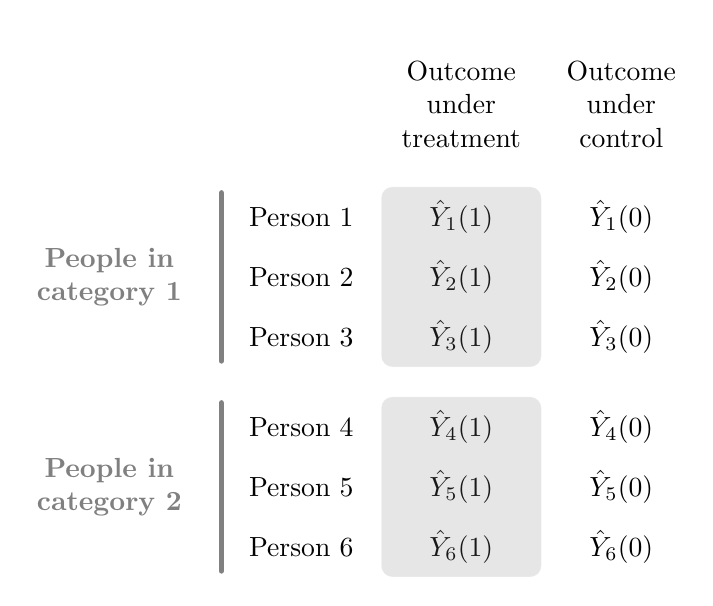
\begin{tikzpicture}[x = .8in, y = .3in, every node/.style={anchor = center}]
\node at (0,-4) {};
\node at (0,2) {};
\node at (0,-1) {Person 1};
\node at (0,-2) {Person 2};
\node at (0,-3) {Person 3};
\node at (0,-4.5) {Person 4};
\node at (0,-5.5) {Person 5};
\node at (0,-6.5) {Person 6};
\node[font = \bf, gray, align = center] at (-1.2,-2) {People in\\category 1};
\node[font = \bf, gray, align = center] at (-1.2,-5.5) {People in\\category 2};
\draw[line cap = round, gray, line width = 2pt] (-.5,-.6) -- (-.5,-3.4);
\draw[line cap = round, gray, line width = 2pt] (-.5,-4.1) -- (-.5,-6.9);
\node[anchor = south, align = center] at (1,0) {Outcome\\under\\treatment};
\node[anchor = south, align = center] at (2,0) {Outcome\\under\\control};
%%
\node at (2,-1) {$\hat{Y}_1(0)$};
\node at (1,-2) {$\hat{Y}_2(1)$};
\node at (1,-3) {$\hat{Y}_3(1)$};
\node at (2,-4.5) {$\hat{Y}_4(0)$};
\node at (1,-5.5) {$\hat{Y}_5(1)$};
\node at (2,-6.5) {$\hat{Y}_6(0)$};
%%
\node at (1,-1) {$\hat{Y}_1(1)$};
\node at (2,-2) {$\hat{Y}_2(0)$};
\node at (2,-3) {$\hat{Y}_3(0)$};
\node at (1,-4.5) {$\hat{Y}_4(1)$};
\node at (2,-5.5) {$\hat{Y}_5(0)$};
\node at (1,-6.5) {$\hat{Y}_6(1)$};
%%
\only<5->{
\draw[color = white, fill = gray, opacity = .2, rounded corners] (.5,-3.5) rectangle (1.5,-.5);
\draw[color = white, fill = gray, opacity = .2, rounded corners] (.5,-7) rectangle (1.5,-4);
}
\end{tikzpicture}}
};
% End predicted science table
\node<4->[anchor = south, font = \small] (predicted_label) at (predicted.north) {Predict the whole table};
\draw<4->[gray, line width = 1.2pt, line cap = round] (predicted_label.south west) -- (predicted_label.south east);
\node<4-5>[gray, font = \footnotesize, align  = right, anchor = south east] at (1,0) {Robins 1986\\Hahn 1998};
% Begin problem
\node<6->[anchor = south, font = \small] (problem) at (.5,.35) {Problem: Optimization for the wrong task};
\draw<6->[gray, line width = 1.2pt, line cap = round] (problem.south west) -- (problem.south east);
\node<7->[align = center, font = \footnotesize] at (.25,.25) {Prediction error over\\\bgray{observed}\\cases};
\node<8->[align = center, font = \footnotesize] at (.5,.25) {vs};
\node<8->[align = center, font = \footnotesize] at (.75,.25) {Prediction error over\\\bgray{all}\\cases};
\end{tikzpicture}
\end{frame}

\begin{frame}
\begin{tikzpicture}[x = \textwidth, y = .9\textheight]
\node at (0,0)  {};
\node at (1,1) {};
\node[anchor = north] (solution) at (.5,.95) {Solution: Reweight errors to approximate the correct task};
\draw[gray, line width = 1.2pt, line cap = round] (solution.south west) -- (solution.south east);
\node<6->[anchor = north west, font = \small] at (0,.8) {Estimated bias:};
\node<6->[align = left, anchor = north west, font = \small] at (.25,.81) {Mean($\hat{Y}_i - Y_i$) with\\inverse probability of treatment weights};
% Table illustrating IPTW
\node<2-6>[anchor = north west] (factual) at (.1,.65) {
\scalebox{.7}{\begin{tikzpicture}[x = .8in, y = .3in, every node/.style={anchor = center}]
\node at (0,-4) {};
\node at (0,2) {};
\node at (0,-1) {Person 1};
\node at (0,-2) {Person 2};
\node at (0,-3) {Person 3};
\node at (0,-4.5) {Person 4};
\node at (0,-5.5) {Person 5};
\node at (0,-6.5) {Person 6};
\node[font = \bf, gray, align = center] at (-1.2,-2) {People in\\category 1};
\node[font = \bf, gray, align = center] at (-1.2,-5.5) {People in\\category 2};
\draw[line cap = round, gray, line width = 2pt] (-.5,-.6) -- (-.5,-3.4);
\draw[line cap = round, gray, line width = 2pt] (-.5,-4.1) -- (-.5,-6.9);
\node[anchor = south, align = center] at (1,0) {Prediction\\under\\treatment};
\node at (1,-1) {$\hat{Y}_1(1)$};
\node at (1,-2) {$\hat{Y}_2(1)$};
\node at (1,-3) {$\hat{Y}_3(1)$};
\node at (1,-4.5) {$\hat{Y}_4(1)$};
\node at (1,-5.5) {$\hat{Y}_5(1)$};
\node at (1,-6.5) {$\hat{Y}_6(1)$};
\node<3->[anchor = south, align = center] at (2,0) {Outcome\\under\\treatment};
\node<3-> at (2,-1) {?};
\node<3-> at (2,-2) {$Y_2$};
\node<3-> at (2,-3) {$Y_3$};
\node<3-> at (2,-4.5) {?};
\node<3-> at (2,-5.5) {$Y_5$};
\node<3-> at (2,-6.5) {?};
\node<4->[anchor = south, align = center] at (3,0) {Error};
\node<4-> at (3,-1) {?};
\node<4-> at (3,-2) {$\hat{Y}_2(1) - Y_2$};
\node<4-> at (3,-3) {$\hat{Y}_3(1) - Y_3$};
\node<4-> at (3,-4.5) {?};
\node<4-> at (3,-5.5) {$\hat{Y}_5(1) - Y_5$};
\node<4-> at (3,-6.5) {?};
\node<5->[anchor = south, align = center] at (4,0) {Weight\\on error};
\node<5-> at (4,-2) {3 / 2};
\node<5-> at (4,-3) {3 / 2};
\node<5-> at (4,-5.5) {$3$};
\draw[color = white, fill = gray, opacity = .2, rounded corners] (.5,-3.5) rectangle (1.5,-.5);
\draw[color = white, fill = gray, opacity = .2, rounded corners] (.5,-7) rectangle (1.5,-4);
\end{tikzpicture}}
};
% End table illustrating IPTW
% Begin doubly robust
\node<7->[anchor = north west, align = center, font = \small] at (0,.65) {New Estimate:};
\node<7->[anchor = north west, font = \small] at (.25,.65) {(Original Estimate) $-$ (Estimated Bias)};
\node<8->[anchor = north east, font = \footnotesize, align = right] at (1,.65) {Doubly\\Robust\\Estimation};
\node<8-12>[anchor = south east, font = \footnotesize, align = right, gray] at (1,0) {Robins, Rotnitzky, \& Zhao 1994\\Bang \& Robins 2005};
\node<9>[anchor = north] at (.5,.5) {\includegraphics[width = \textwidth]{figures/sim_x1mx0_0}};
\node<10>[anchor = north] at (.5,.5) {\includegraphics[width = \textwidth]{figures/sim_x1mx0_1}};
\node<11>[anchor = north] at (.5,.5) {\includegraphics[width = \textwidth]{figures/sim_x1mx0_2}};
\node<12>[anchor = north] at (.5,.5) {\includegraphics[width = \textwidth]{figures/sim_x1mx0_3}};
% Begin DML
\node<13->[anchor = north west, font = \small] at (0,.45) {Even better:};
\node<14->[anchor = north west, font = \small] (sample_split_A) at (.25,.46) {--- Learn $\hat{Y}_i$ in sample A};
\node<14->[anchor = north west, font = \small] (sample_split_B) at (sample_split_A.south west) {--- Estimate bias in sample B};
\node<15->[anchor = north west, font = \small] (sample_split_C) at (sample_split_B.south west) {--- Cross fit: Swap roles and average};
\node<17> at (.5,.5) {\includegraphics[width = \textwidth]{figures/sim_cross_fitting_slide_0}};
\node<18> at (.5,.5) {\includegraphics[width = \textwidth]{figures/sim_cross_fitting_slide_1}};
\node<19> at (.5,.5) {\includegraphics[width = \textwidth]{figures/sim_cross_fitting_slide_2}};
\node<20> at (.5,.5) {\includegraphics[width = \textwidth]{figures/sim_cross_fitting_slide_3}};
\node<21->[anchor = north east, font = \footnotesize, align = right] at (1,.45) {Double\\Machine\\Learning};
\node<13-16,21>[anchor = south east, font = \footnotesize, align = right, gray] at (1,0) {Chernozhukov et al. 2018\\Bickel 1982};
\node<22->[red, draw, rounded corners, line width = 2pt, font = {\footnotesize\bf}, rotate = 20] at (.3,.1) {So complicated!};
\end{tikzpicture}
\end{frame}

\begin{frame}[t,fragile]
\includegraphics[width = .8\textwidth]{figures/gapclosing_package}

\begin{scriptsize}
\begin{verbatim}
estimate <- gapclosing(
  data = simulated_data,
  outcome_formula = formula(outcome ~ category + confounder),
  treatment_formula = formula(treatment ~ category + confounder),
  category_name = "category",
  counterfactual_assignments = 1,
  outcome_algorithm = "ranger",
  treatment_algorithm = "ranger",
  sample_split = "cross_fit",
  se = T
)
\end{verbatim}

\begin{verbatim}
        description estimate   se ci.min ci.max
        Factual gap     2.14 0.40   1.36    2.9
 Counterfactual gap     0.67 0.44  -0.19    1.5
 \end{verbatim}
 \end{scriptsize}
\end{frame}

\begin{frame}
How should one interpret results?
\end{frame}

\begin{frame}
\begin{tikzpicture}[x = \textwidth, y = .9\textheight]
\node at (0,0) {};
\node at (1,1) {};
\node[anchor = north west] at (0,.95) {Interpret with respect to a \bgray{target trial} \begin{scriptsize}(Hern\'an \& Robins 2016)\end{scriptsize}};
\node<6->[anchor = north west] (local) at (0,.65) {Local intervention};
\node<2->[anchor = north west, font = \footnotesize] at (0,.55) {1.};
\node<3->[anchor = north west, font = \footnotesize] at (0,.5) {2.};
\node<4->[anchor = north west, font = \footnotesize, align = left] at (0,.45) {3.};
\node<2->[anchor = north west, font = \footnotesize] at (.03,.55) {Sample $\mathcal{S}$ from the population};
\node<3->[anchor = north west, font = \footnotesize] at (.03,.5) {Assign treatment $T = 1$ to $\mathcal{S}$};
\node<4->[anchor = north west, font = \footnotesize, align = left] at (.03,.45) {Observe the disparity\\across categories $X$};
\node<5->[anchor = north west, font = \footnotesize, align = left] at (0,.3) {Goal: };
\node<5->[anchor = north west, font = \footnotesize, align = left] at (.1,.3) {Expected result over\\hypothetical samples $\mathcal{S}$};
\node<12->[anchor = north west, font = \footnotesize, align = left] at (0,.15) {Difficulty:};
\node<12->[anchor = north west, font = \footnotesize, align = left] at (.15,.15) {Causal inference};
%%%%%%%
\node<7->[anchor = north west] (global) at (.55,.65) {Global intervention};
\node<8->[anchor = north west, font = \footnotesize] at (.55,.55) {1.};
\node<9->[anchor = north west, font = \footnotesize] at (.55,.5) {2.};
\node<10->[anchor = north west, font = \footnotesize, align = left] at (.55,.45) {3.};
\node<8->[anchor = north west, font = \footnotesize] at (.58,.55) {Take the entire population $\mathcal{P}$};
\node<9->[anchor = north west, font = \footnotesize] at (.58,.5) {Assign treatment $T = 1$ to $\mathcal{P}$};
\node<10->[anchor = north west, font = \footnotesize, align = left] at (.58,.45) {Observe the disparity\\across categories $X$};
\node<11->[anchor = north west, font = \footnotesize, align = left] at (.55,.3) {Goal: };
\node<11->[anchor = north west, font = \footnotesize, align = left] at (.65,.3) {Result of this procedure};
\node<12->[anchor = north west, font = \footnotesize, align = left] at (.55,.15) {Difficulty:};
\node<12->[anchor = north west, font = \footnotesize, align = left] (diff2a) at (.7,.15) {Causal inference};
\node<13->[anchor = north west, font = \footnotesize, align = left] at (diff2a.south west) {Equilibrium dynamics};
% Tension
\draw<14->[line width = 2.5pt] (.25,.7) -- (.75, .7);
\node<14->[font = \Huge] at (.25,.7) {$\bullet$};
\node<14->[font = \Huge] at (.75,.7) {$\bullet$};
\node<15>[anchor = south, align = right, font = \footnotesize, gray] at (.7,.77) {Policy-relevant?};
\draw<15>[->, thick, gray] (.7,.77) -- (.7,.72);
\node<16>[anchor = south, align = right, font = \footnotesize, gray] at (.3,.77) {Policy-relevant.};
\draw<16>[->, thick, gray] (.3,.77) -- (.3,.72);
\end{tikzpicture}
\end{frame}

\begin{frame}
\Huge
Empirical Examples
\end{frame}

% EXAMPLE 1: ECONOMIC MOBILITY
\begin{frame}
\begin{tikzpicture}[x = \textwidth, y = \textheight]
\node at (0,0) {};
\node at (1,1) {};
\node[anchor = west] at (0,.95) {\bblue{Empirical Example 1}: Economic Mobility};
% DAG
\onslide<1-4>{
\node (x) at (.2,.6) {$X$};
\node[anchor = east, font = \footnotesize, align = center] (x_label) at (x.west) {Father's\\Social Class};
\node[anchor = north, font = \scriptsize, align = center, gray] at (x_label.south) {Professional\\or\\Working Class};
\node (y) at (.8,.6) {$Y$};
\node[font = \footnotesize, align = center, anchor = west] at (y.east) {Your\\Income};
\draw[<->, thick] (x) to[out = 90, in = 90] (y);
}
\onslide<2-4>{
\node[anchor = south, font = \footnotesize, align = center] at (t.north) {Your\\Social Class};
\node (t) at (.5,.6) {$T$};
\draw<2-3>[->, thick] (x) -- (t);
\draw[->, thick] (t) -- (y);
}
\onslide<3-4>{
\node (l) at (.2,.4) {$\vec{L}$};
\draw[<->, thick] (x) -- (l);
\draw<3>[->, thick] (l) -- (t);
\draw[->, thick] (l) to[bend right = 15] (y);
\node[anchor = north, font = \footnotesize, align = left] at (l.south) {Race, Sex,\\Age, Education};
}
\onslide<4>{
\node[font = {\scriptsize\bf}, blue]  (intervention) at (.35,.5) {Intervention};
\draw[->, thick, snake = zigzag, blue, line before snake = 10pt, line after snake = 10pt, segment length = 4pt] (intervention) -- (t);%(.43,.52) -- (.48,.58);
}
% Result
\node<5>[anchor = south] at (.5,.1) {\includegraphics[width = \textwidth]{figures/empirical_example_slide_0}};
\node<6>[anchor = south] at (.5,.1) {\includegraphics[width = \textwidth]{figures/empirical_example_slide_1}};
\node<7>[anchor = south] at (.5,.1) {\includegraphics[width = \textwidth]{figures/empirical_example_slide_2}};
\node<8-9>[anchor = south] at (.5,.1) {\includegraphics[width = \textwidth]{figures/empirical_example_slide_3}};
\node<9>[anchor = east, draw, rounded corners] at (.97,.87) {\texttt{plot\_two\_categories()}};
\end{tikzpicture}
\end{frame}

% EXAMPLE 2: OCCUPATIONAL SEGREGATION
\begin{frame}
\begin{tikzpicture}[x = \textwidth, y = \textheight]
\node at (0,0) {};
\node at (1,1) {};
\node[anchor = west] at (0,.95) {\bblue{Empirical Example 2}: Racial Disparities in Health};
% DAG
\onslide<1-4>{
\node (x) at (.2,.6) {$X$};
\node[anchor = east, font = \footnotesize, align = center] (x_label) at (x.west) {Race};
\node (y) at (.8,.6) {$Y$};
\node[font = \footnotesize, align = center, anchor = west] at (y.east) {Onset of\\work-limiting\\disability};
\draw[<->, thick] (x) to[out = 90, in = 90] (y);
}
\onslide<2-4>{
\node[anchor = south, font = \footnotesize, align = center] at (t.north) {Occupation};
\node (t) at (.5,.6) {$T$};
\draw<2-3>[->, thick] (x) -- (t);
\draw[->, thick] (t) -- (y);
}
\onslide<3-4>{
\node (l) at (.2,.4) {$\vec{L}$};
\draw[<->, thick] (x) -- (l);
\draw<3>[->, thick] (l) -- (t);
\draw[->, thick] (l) to[bend right = 15] (y);
\node[anchor = north, font = \footnotesize, align = left] at (l.south) {Sex,\\Age, Education\\Foreign born,\\Lagged outcome,\\Lagged health};
}
\onslide<4>{
\node[font = {\scriptsize\bf}, blue]  (intervention) at (.35,.5) {Intervention};
\draw[->, thick, snake = zigzag, blue, line before snake = 10pt, line after snake = 10pt, segment length = 4pt] (intervention) -- (t);
}
% Result
\node<5>[anchor = south] at (.5,.1) {\includegraphics[width = \textwidth]{figures/segregation_slide_0}};
\node<6>[anchor = south] at (.5,.1) {\includegraphics[width = \textwidth]{figures/segregation_slide_1}};
\node<7>[anchor = south] at (.5,.1) {\includegraphics[width = \textwidth]{figures/segregation_slide_2}};
\node<8>[anchor = south] at (.5,.1) {\includegraphics[width = \textwidth]{figures/segregation_slide_3}};
\end{tikzpicture}
\end{frame}

\begin{frame}
\Huge
Discussion
\end{frame}

\begin{frame}{Gap closing estimands}
\begin{itemize}
\item Define the goal
\begin{itemize}
\item two target populations
\item hypothetical intervention
\end{itemize}
\item Make causal assumptions
\begin{itemize}
\item draw a DAG
\end{itemize}
\item Estimate
\begin{itemize}
\item fit an outcome model
\item change the treatment
\item predict for everyone
\item average within the populations
\end{itemize}
\end{itemize}
\end{frame}

\begin{frame}

Now try it! \vskip .1in
\bref{https://ilundberg.github.io/gapclosing/github_doc/_book/index.html}{ilundberg.github.io/gapclosing} \vskip .3in
Ian Lundberg\\
\bref{https://www.ianlundberg.org/}{ianlundberg.org} \\
\bref{mailto:ilundberg@cornell.edu}{ilundberg@cornell.edu}

\end{frame}

\end{document}

